\documentclass[slovak]{beamer}
\usetheme{beaver}

\usepackage[T1]{fontenc}
\usepackage[utf8]{inputenc}
\usepackage{graphicx}

\newcommand{\jl}{$\frac{}{}$} 

\title{Caver Analyst XML projekt}
\date{2014}
\author{
	Jan Štourač, Henrich Lauko, Jiří Novotný, Karel Kubíček
}


\begin{document}

\begin{frame}
	\titlepage
\end{frame}

\begin{frame}
\frametitle{Caver Analyst}
	
\includegraphics[width=\linewidth]{caver_start.jpg}
\end{frame}

\begin{frame}
\frametitle{Caver Analyst}
	\begin{itemize}
		\item bioinformatický nástroj určený pro analýzu tunelôv v proteinech
		\item široké využití v komunitě biochemikú a proteinových inženýrú 
		\item grafická nadstavba výpočetního jádra Caver (Chovancová at el. 2012)
		\item vlastní vizualizační jádro
	\end{itemize}
\end{frame}

\begin{frame}
\frametitle{Caver Application}
	\begin{center}
		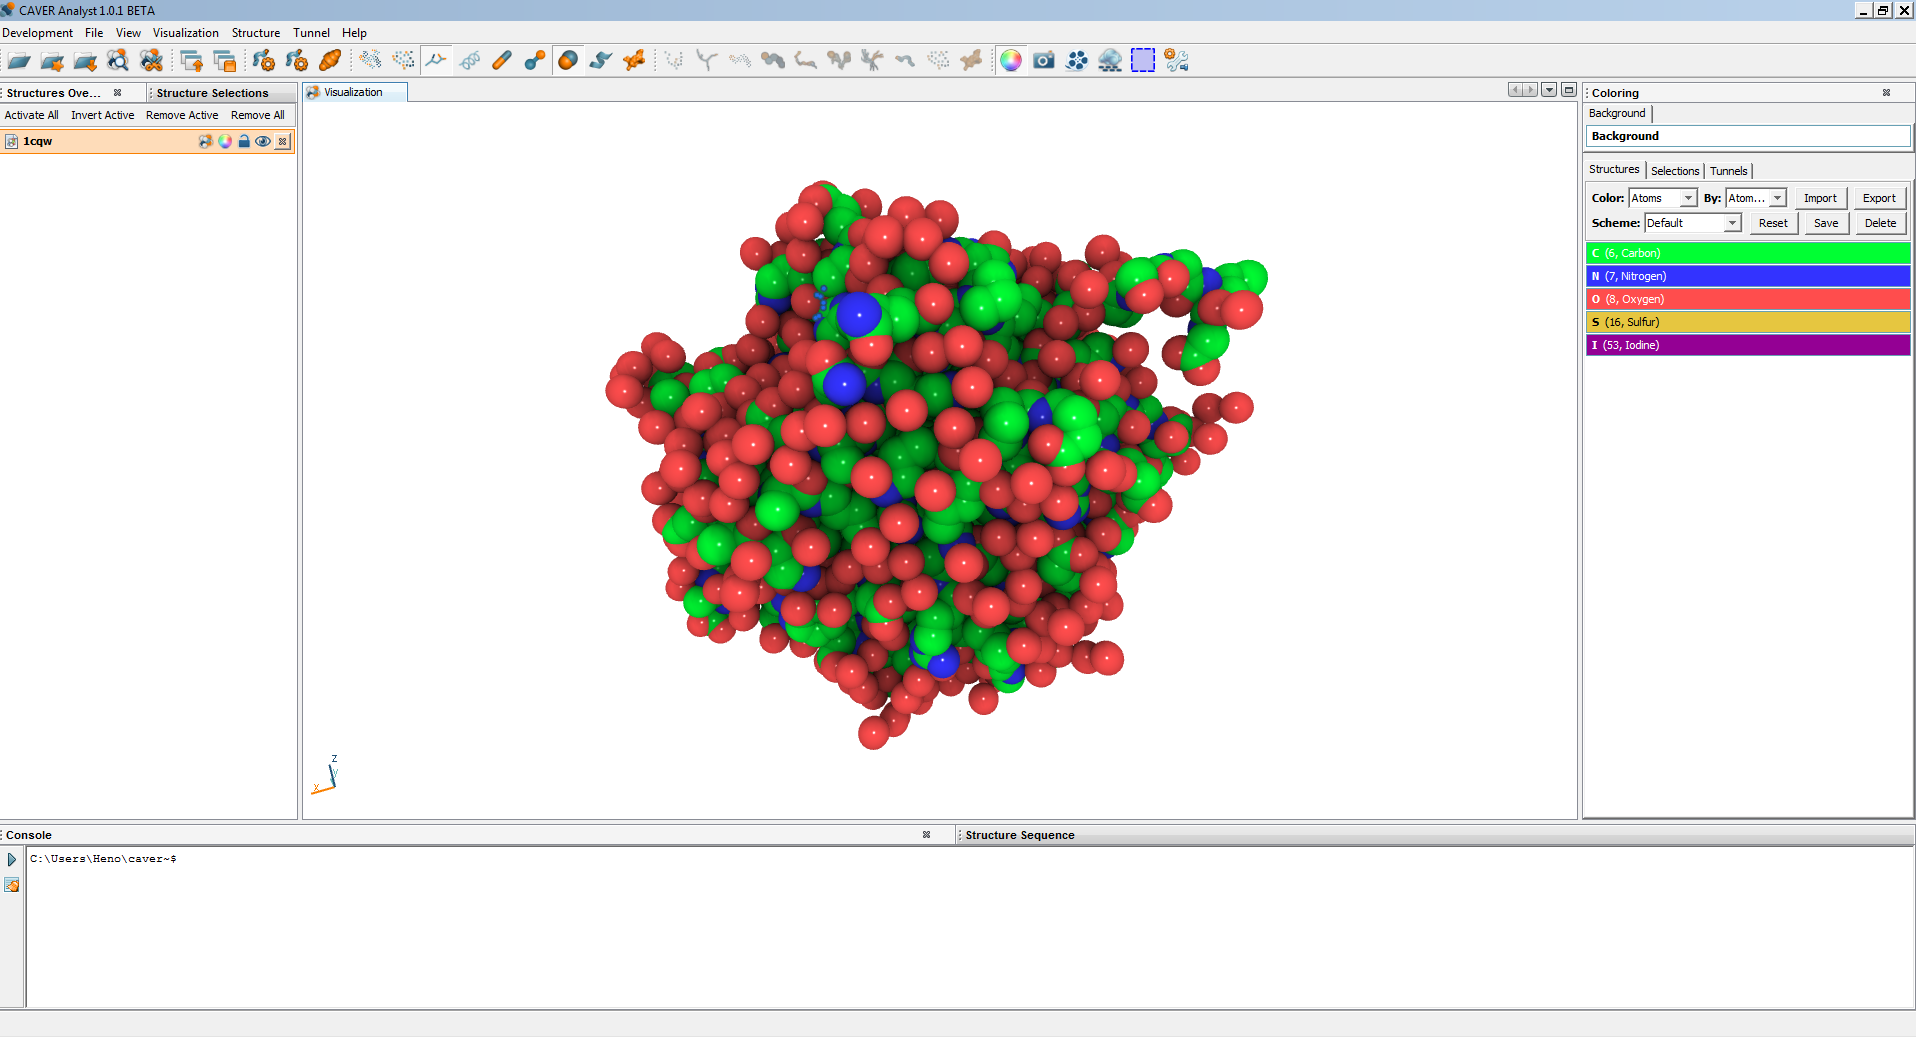
\includegraphics[width=\linewidth]{caver.png}
	\end{center}
\end{frame}



\begin{frame}
\frametitle{Ciele}
	\begin{itemize}
		\item uživatelská barevná schémata
		\begin{itemize}
			\item efektivní ukládání schémat do XML souboru
			\item podpora importu a exportu
			\item přívětivé uživatelské rozhraní
		\end{itemize}
		\item úprava XML s globálním nastavením aplikace
	\end{itemize}
\end{frame}

\begin{frame}
\frametitle{Organizace projektu}
	\begin{itemize}
		\item Rozdělení úloh:
		\begin{itemize}
			\item Backend - Jan Štourač
			\item GUI - Henrich Lauko
			\item XML struktura a XSD - Karel Kubíček
			\item Globální nastavení - Jiří Novotný
		\end{itemize}
		\item Využití interního svn repozitáře pro zdrojový kód
		\item Wiki na github.com
		\begin{itemize}
			\item Zakomponováno do interní dokumentace
		\end{itemize}
		\item kód dokumentován pomocí JavaDoc
	\end{itemize}
\end{frame}

\begin{frame}
\frametitle{Proces vývoje}
	\begin{itemize}
		\item 21. 3. - stretnutie o možnostiach práce v Caveri a rozdelenie úloh
		\item 22.3. - 11.4. - zorientovanie sa v Caveri a práca na vývoji
		\item 12.4. - 20.4. - testovanie a drobné úpravy
		\item 21.4. - 27.4. - dokončovanie dokumentácie a wiki stránok
		\item 4.5. - predpokladané ukončenie práce na projekte
	\end{itemize}
\end{frame}

\begin{frame}
\frametitle{Backend}
	\begin{itemize}
		\item návrh a implementace API pro práci s barevnými schématy
		\begin{itemize}
			\item globální manažer schémat pro celou aplikaci
		\end{itemize}
		\item oddělení systémových a uživatelských schémat
		\item notifikace o GUI při změnách
	\end{itemize}
\end{frame}

\begin{frame}
\frametitle{XML color schémy}
	\begin{itemize}
		\item návrh reprezentácie farebných schém v XML
		\item rodelenie default a user schém
		\item ukládání schémat pomocí rozdílú
		\item kontrolná XSD schéma
		\item synchronizácia schém cez projektovú stránku
	\end{itemize}
\end{frame}

\begin{frame}
\frametitle{XML color GUI}
	\begin{itemize}
		\item ukazka XML / XSD (TODO obrazok)
	\end{itemize}
\end{frame}

\begin{frame}
\frametitle{Color schémy GUI}
	\begin{itemize}
		\item implementoval Henrich Lauko
		\item návrh uživatelského rozhrania
		\item rozdelenie panelov do default a user profilov
		\item riešený problém synchronizácie všetkých panelov pracujúcich s farebnými schémami
	\end{itemize}
\end{frame}

\begin{frame}
\frametitle{Color schémy GUI}
	\frametitle{Color schémy GUI}
	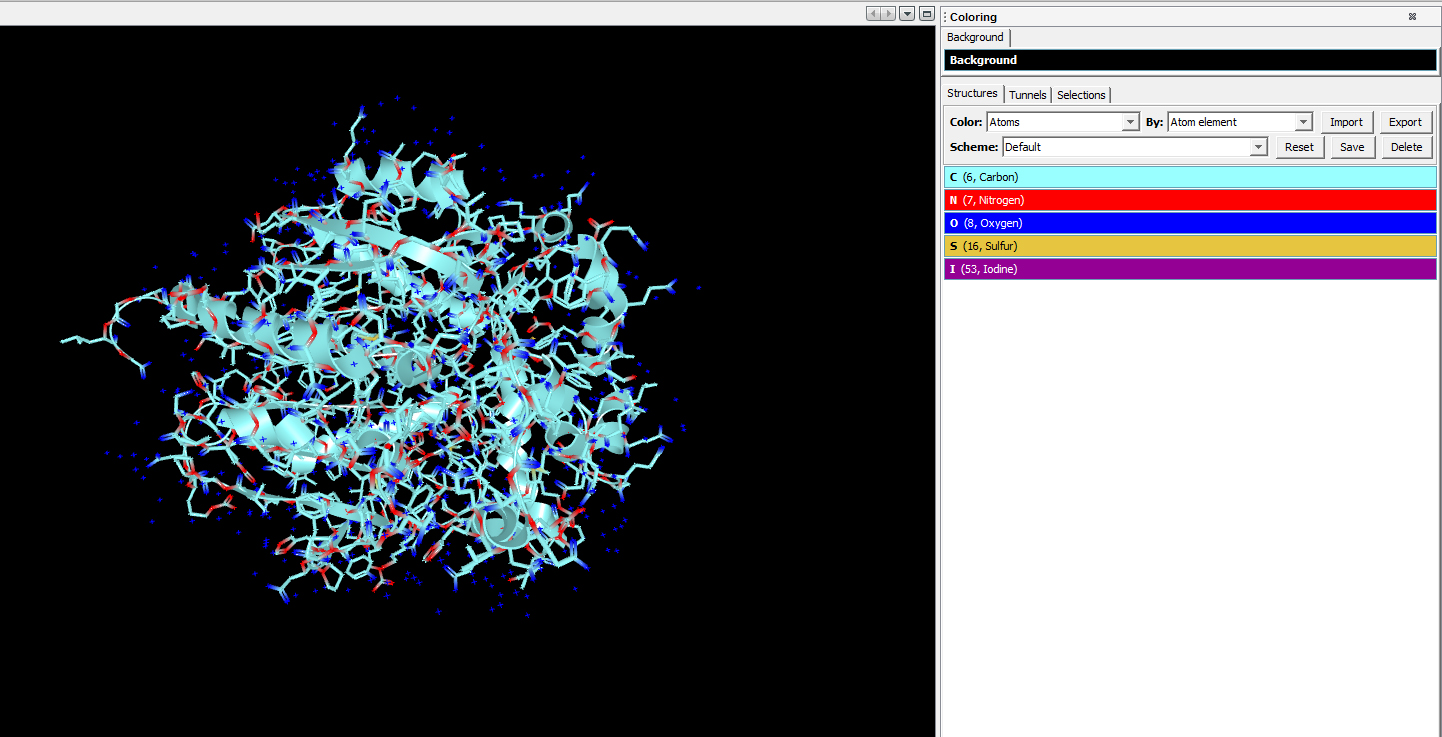
\includegraphics[width=\linewidth]{colorpanel.jpg}
\end{frame}

\begin{frame}
\frametitle{Global settings}
	\begin{itemize}
		\item Jirka slide
	\end{itemize}
\end{frame}

\begin{frame}
\frametitle{Zhodnocení projektu}
	\begin{itemize}
		\item vylepšená podpora barevných schémat
		\item možnost importu a exportu uživatelsky definovaných schémat
		\item zpřístupnění XSD souboru pro manuální validaci
		\item nové přívětivé uživatelské rozhraní
		\item snadná rozšiřitelnost aplikace o další barvitelné prvky
		\begin{itemize}
			\item jednoduše využitelné veřejné API
			\item notifikace jednotlivých komponent
		\end{itemize}
		\item vylepšená správa globálního nastavení aplikace 
	\end{itemize}
\end{frame}

\end{document}
